This section provides an overview of the Fiducial Career Display. A table will be constructed upon which the top surface will consist of a video display. The display will recognize specific objects played on top of it and will be able to track their movement across the surface if moved or rotated. Object recognition will be dependent on uniquely shaped or patterned markers placed on the bottom of the object. For objects placed on the surface of the table that do not contain a recognized pattern (like a fingertip), the table will treat as user interaction (touch gesture). Each marker will display the details including text, image, or videos about that career.
\subsection{Features \& Functions}
Hardware features:
\begin{itemize}
\item A semi-transparent acrylic board that make the table top as well as interactive display.
\item An infrared camera used to capture the input from the user.
\item A short throw projector mounted below the table to provide the interactive display.
\item A computer to run the recognition and application softwares.
\item A Fiducial marker that will represent a career. When a marker is placed on the table, an interface will appear to allow the user to page through different details about that career.
\end{itemize}


Software Features:
\begin{itemize}
\item Movable modular interface.
\item Automatic orientation based on position on table.
\item Navigable content.
\item Logo screen when not engaged.
\item Transitions in and out when marker is introduced and removed.
\item Track type of markers on the table.
\end{itemize}

\subsection{External Inputs \& Outputs}

\begin{table}[H]
\centering
\caption{Input \& Output}
\label{input}
\begin{tabular}{|l|l|l|}
\hline
Name            & Description                                                                                                              & Use                                                                                                      \\ \hline
Input           &                                                                                                                          &                                                                                                          \\ \hline
Fiducial Marker & \begin{tabular}[c]{@{}l@{}}Fiducial markers which can be tracked from \\ a camera and interpreted using software.\end{tabular} & \begin{tabular}[c]{@{}l@{}}Place on top of the table for \\ activating career choice menu\end{tabular} \\ \hline
Finger touch    & Human finger on the table surface                                                                                        & \begin{tabular}[c]{@{}l@{}}Use to select and interact\\ with the menu\end{tabular}                   \\ \hline
Output          &                                                                                                                          &                                                                                                          \\ \hline
Display         & \begin{tabular}[c]{@{}l@{}}A semi-transparent tabletop capable \\ of display\end{tabular}                              & \begin{tabular}[c]{@{}l@{}}Projected the screen to the \\ table surface\end{tabular}                    \\ \hline
Sound           & Audio source                                                                                                             & Play on input and media request                                                                                  \\ \hline
\end{tabular}
\end{table}

\subsection{Product Interfaces}

\begin{figure}[H]
	\centering
   	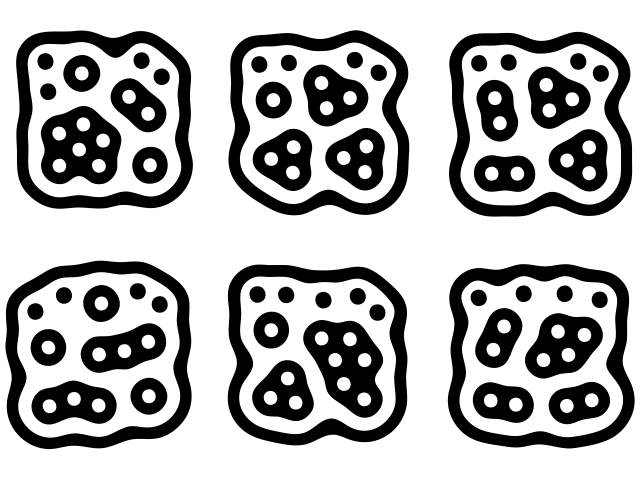
\includegraphics[width=0.6\textwidth]{images/reactivision02}
    \caption{Fiducial pattern examples}
\end{figure}

\begin{figure}[H]
	\centering
   	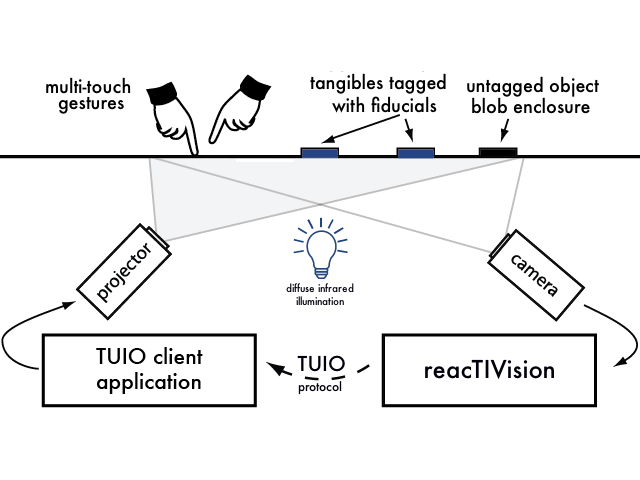
\includegraphics[width=0.9\textwidth]{images/reactivision03}
    \caption{Table concept }
\end{figure}

\begin{figure}[H]
	\centering
   	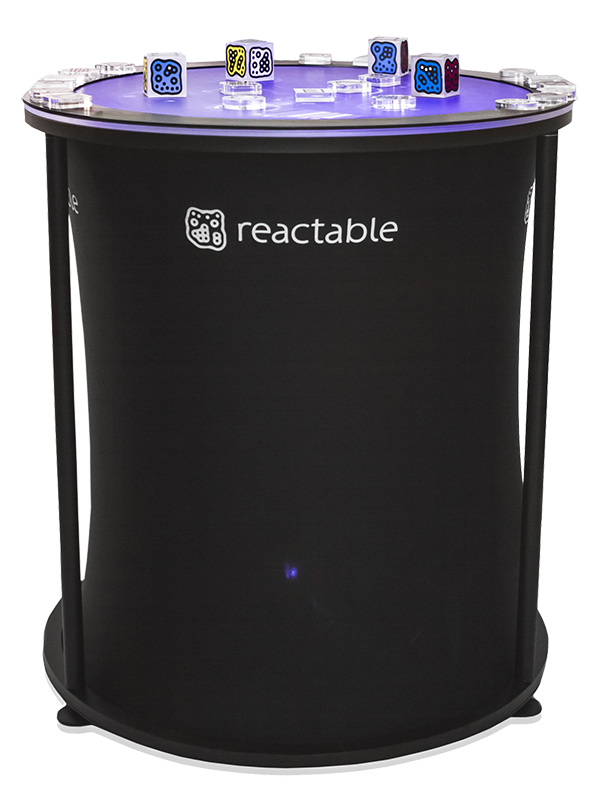
\includegraphics[width=0.4\textwidth]{images/ReacTable-live-6-instrument}
    \caption{Round table concept}
\end{figure}

\begin{figure}[H]
	\centering
   	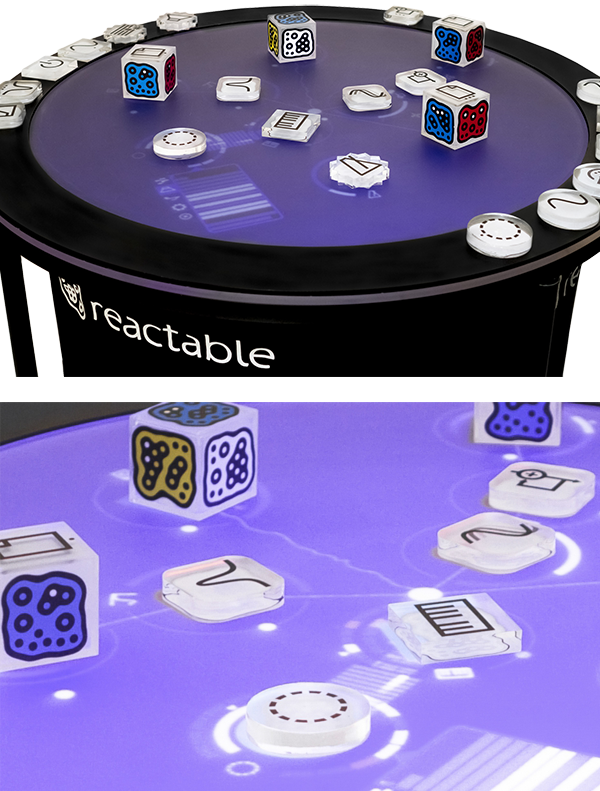
\includegraphics[width=0.5\textwidth]{images/ReacTable-instrument-detail1}
    \caption{Round table concept \cite{concept2}}
\end{figure}
